% BSD 3-Clause License
%
% Copyright (c) 2023, 2024 Quux System and Technology. All rights reserved.
%
% Redistribution and use in source and binary forms, with or without
% modification, are permitted provided that the following conditions are met:
%
% 1. Redistributions of source code must retain the above copyright notice, this
%    list of conditions and the following disclaimer.
%
% 2. Redistributions in binary form must reproduce the above copyright notice,
%    this list of conditions and the following disclaimer in the documentation
%    and/or other materials provided with the distribution.
%
% 3. Neither the name of the copyright holder nor the names of its
%    contributors may be used to endorse or promote products derived from
%    this software without specific prior written permission.
%
% THIS SOFTWARE IS PROVIDED BY THE COPYRIGHT HOLDERS AND CONTRIBUTORS "AS IS"
% AND ANY EXPRESS OR IMPLIED WARRANTIES, INCLUDING, BUT NOT LIMITED TO, THE
% IMPLIED WARRANTIES OF MERCHANTABILITY AND FITNESS FOR A PARTICULAR PURPOSE ARE
% DISCLAIMED. IN NO EVENT SHALL THE COPYRIGHT HOLDER OR CONTRIBUTORS BE LIABLE
% FOR ANY DIRECT, INDIRECT, INCIDENTAL, SPECIAL, EXEMPLARY, OR CONSEQUENTIAL
% DAMAGES (INCLUDING, BUT NOT LIMITED TO, PROCUREMENT OF SUBSTITUTE GOODS OR
% SERVICES; LOSS OF USE, DATA, OR PROFITS; OR BUSINESS INTERRUPTION) HOWEVER
% CAUSED AND ON ANY THEORY OF LIABILITY, WHETHER IN CONTRACT, STRICT LIABILITY,
% OR TORT (INCLUDING NEGLIGENCE OR OTHERWISE) ARISING IN ANY WAY OUT OF THE USE
% OF THIS SOFTWARE, EVEN IF ADVISED OF THE POSSIBILITY OF SUCH DAMAGE.
%
\begin{recipe}{奶汤大杂烩}

\ingredients

\ingredient{干猪肉皮}{一两五}
\ingredient{胡椒}{三分}
\ingredient{熟猪肚}{一两五}
\ingredient{火腿}{一两}
\ingredient{水豆粉}{六分}
\ingredient{猪肉}{六两}
\ingredient{鲜青菜}{一束}
\ingredient{熟猪舌}{一两五}
\ingredient{干豆粉}{七钱}
\ingredient{料酒}{七钱}
\ingredient{菜油}{一斤半耗四两}
\ingredient{熟猪心}{一两五}
\ingredient{干笋}{一两五}
\ingredient{味精}{三分}
\ingredient{盐}{八分}
\ingredient{鸡蛋}{四个}
\ingredient{鸡松菌}{一两}
\ingredient{特级奶汤}{一斤四两}

\preparation

\step 锅内倒入菜油一斤半烧热,将猪肉皮放入,约五分钟炸软,连锅提起,移放微火上
再浸五分钟,至色为深牙黄色时捞起晾冷,切成一寸长的条块,漂于清水中待用(俗称
响皮)。

\step 干笋洗净,用水浸泡,胀透为度;再每条用手撕成四条,切成二寸的段。然后入沸
水中煮透,去净硫磺质味,再用清汤汆一次,捞出待用。

\step 选用肥膘猪肉二两,洗净去皮,切成二寸长、四分宽的片。鸡蛋(二个)、干豆粉
(五钱)混合调为蛋清豆粉,加盐(二分)与肉片拌匀。锅内菜油烧红,把拌好的肉片放
入
\begin{wrapfigure}[9]{r}{12em}%
\centering%
\vspace{.3125\baselineskip}%
\quad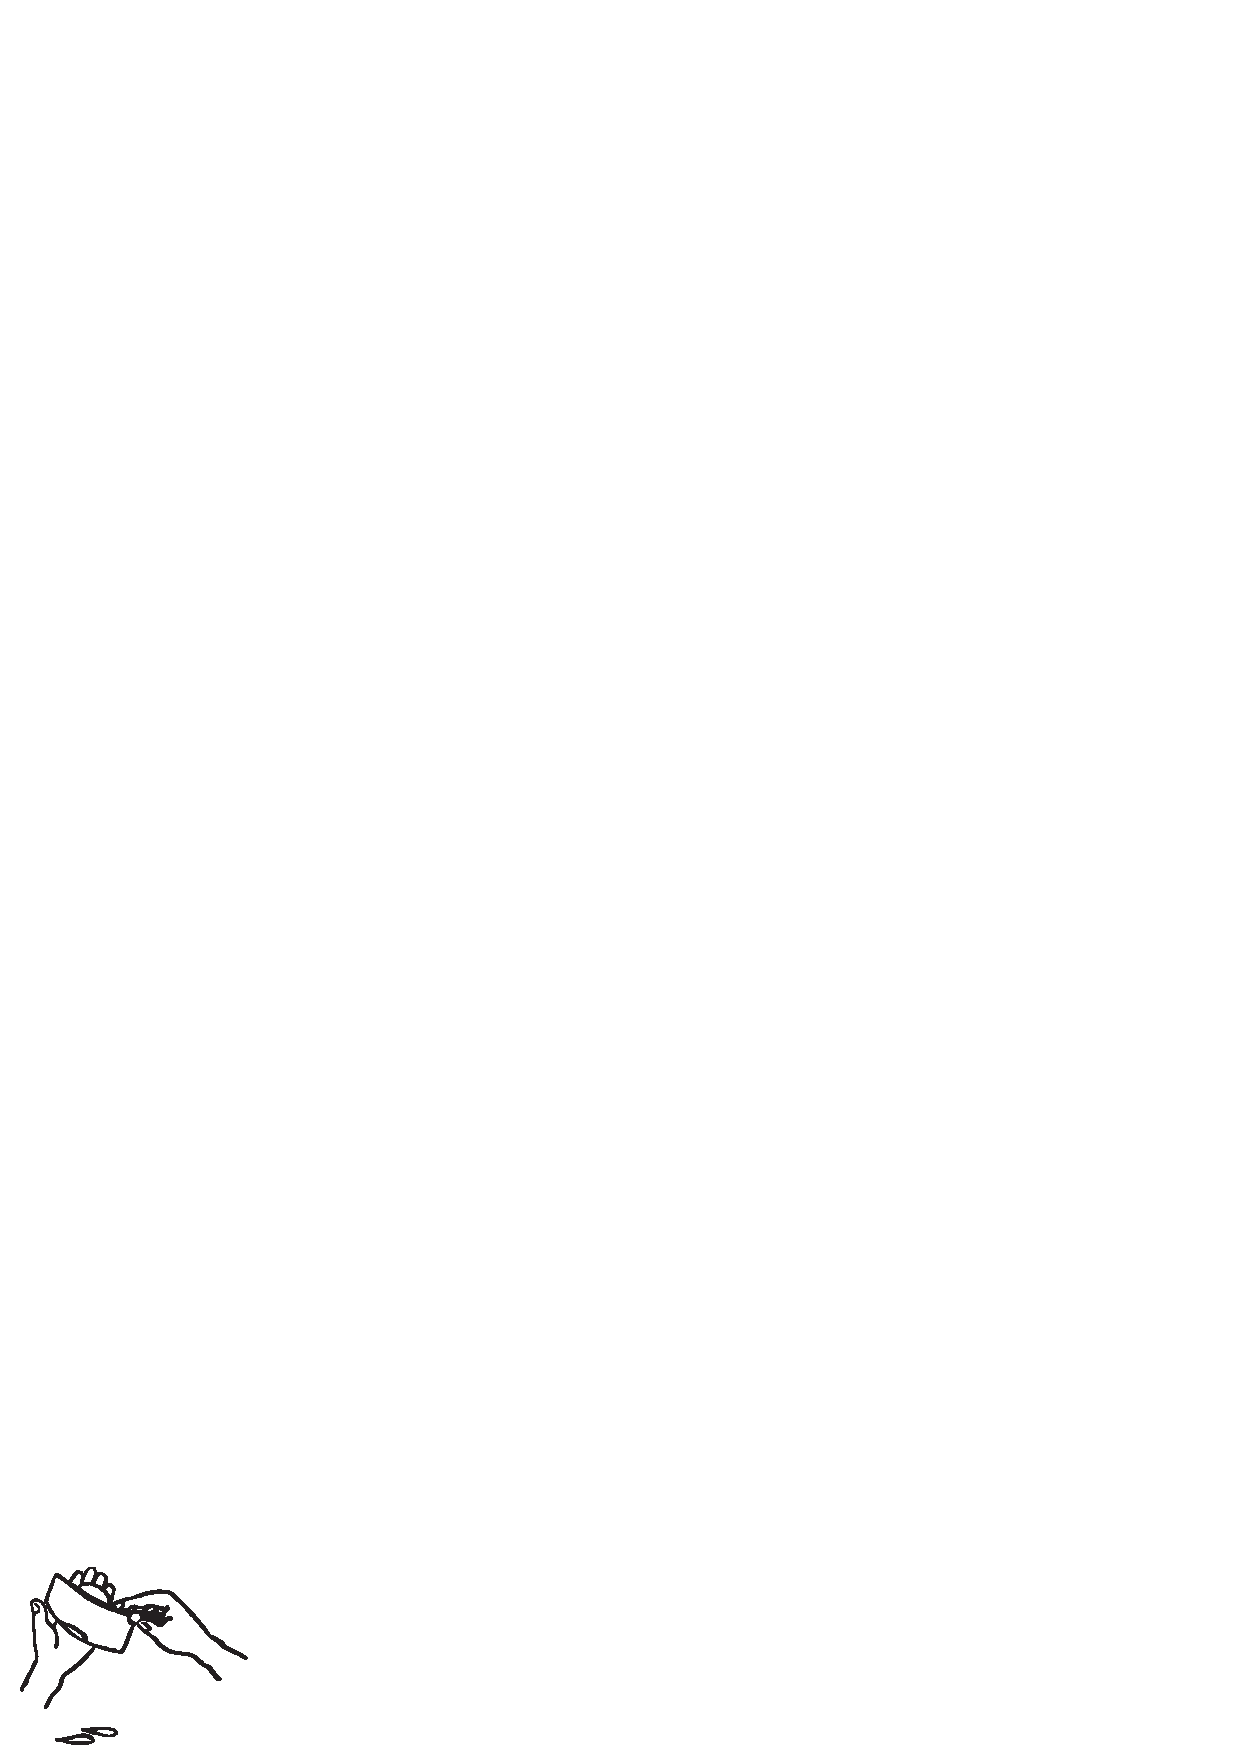
\includegraphics[scale=1]{illustration-001.pdf}%
\vspace{-.1875\baselineskip}%
\caption{尖刀圆子做法}
\label{fig:making-meatballs}
\end{wrapfigure}%
\vbadness=10000%
炸五分钟,至炸成深牙黄色时捞出,晾冷待用(俗称酥肉)。

\step 选用肥瘦相连的猪肉二两,洗净去皮,剁为肉茸,加干豆粉(二钱)、鸡蛋(一个
去壳)、盐(三分)混合调匀,拨一部分摊于左手上面(平摊约四分厚、一寸半宽),右
手持刀斜刮左手的肉茸为上大下小的三角条形(俗称鲫鱼背)共十六条,分开摆于盘内,
入笼蒸十分钟后取出晾冷待用(图\,\ref{fig:making-meatballs}\,俗称尖刀圆子)。

\step 熟猪心、猪舌均切成一寸半长的薄片。

\begin{figure}[h]
\hbadness=10000%
\vbadness=2000%
\vspace{-.6875\baselineskip}%
\begin{subfigure}[h]{\linewidth}%
\centering%

\includegraphics[scale=1]{illustration-002a.pdf}%
\raise1.125\baselineskip%
\hbox{\fsfamily\scalebox{1}[1.142857]{甲}}%
\end{subfigure}%
\vspace{.3125\baselineskip}%
\\%
\parbox{14.75em}{%
	\hspace{4em}
\includegraphics[scale=1]{illustration-002b.pdf}%
	\kern-.625em\raise1.5\baselineskip%
	\hbox{\fsfamily\scalebox{1}[1.142857]{乙}}%
}%
\begin{minipage}{11em}
	\vspace{.25\baselineskip}%
	
\includegraphics[scale=1]{illustration-002c.pdf}%
	\raise1.25\baselineskip%
	\hbox{\fsfamily\scalebox{1}[1.142857]{丙}}%
	\vspace{1.25\baselineskip}%
	\caption{如意蛋卷制作过程}
	\label{fig:fortune-egg-rolls}
	\vspace{1\baselineskip}%
	\begingroup%
	\small%
	\noindent%
	\null\hspace{1.5em}甲、肉丝放入蛋皮两端\\
	\null\hspace{3.5em}1.蛋皮;\hspace{1em}2.肉丝\\
	\null\hspace{1.5em}乙、卷成两卷\\
	\null\hspace{1.5em}丙、如意蛋卷
	\endgroup%
\end{minipage}
\vspace{-.75\baselineskip}%
\end{figure}%

\step 鸡蛋一个,去壳搅散。炒锅烧热,锅中擦净,稍用菜油涂匀,将蛋倾入,以手提耳
锅转动,即摊成蛋皮,稍冷,蛋皮即自行脱落。把肥瘦相连的猪肉二两洗净,剁成细茸,
加入水豆粉、盐、胡椒,调匀后铺于贴锅一面的蛋皮上(如图\,%
\ref{fig:fortune-egg-rolls}\,甲),两端向中央搓裹,成为两卷,中间相连(如图\,%
\ref{fig:fortune-egg-rolls}\,乙),接口处涂少许豆粉粘好。然后平放盘内入笼蒸十
五分钟,取出晾冷,用刀稍斜横切成一寸半宽的小块(俗称如意蛋卷)(如图\,%
\ref{fig:fortune-egg-rolls}\,丙)。

\step 用平底大碗一个,先将汆好的笋条、响皮摆在碗底;次将酥肉逐片摆成圆形,为第
二层;又将尖刀圆子十六条分为每方四条摆成卍字形,为第三层;再将猪心、猪舌像铺瓦
一样分别各摆半个碗,成圆形,为第四层;最后将蛋卷用刀平铲放于上面。再用火腿,把
特级奶汤、味精、料酒灌入摆好的杂烩碗内,入笼蒸二小时取出。再用特级奶汤十两,加
味精、盐,舀入杂烩内。另选绿色鲜菜一束,淘洗烫熟,放入碗内以衬其色即成。

\features

此菜系汤菜合一,味鲜可口,佐酒下饭均宜。

\end{recipe}

% vim: filetype=tex noautoindent nojoinspaces
% vim: fileencoding=utf-8 formatoptions+=m
% vim: textwidth=78 tabstop=4 shiftwidth=4 softtabstop=4
